\chapter{Einleitung}
In diesem ersten Kapitel wird auf die Aufgabenstellung und die Ziele dieser Diplomarbeit eingegangen. 


\section{Zielsetzung und Aufgabenstellung}
Eine allgemeine Beschreibung, die Veranlassung, das Ziel und das Ergebnis dieser Diplomarbeit ist der Inhalt der folgenden Abschnitten.


\subsection{Beschreibung der Diplomarbeit}
Im Rahmen der Diplomarbeit „Echtzeit-Visualisierung von Energiesystemen” soll ein Produkt zur Verwaltung von Energiesystemen erstellt werden. Dabei soll auf die bereits bestehenden Komponenten wie Webserver, Datenbank sowie Grafana Server aufgebaut werden. Der Webserver präsentiert die Verwaltungsanwendung, welche öffentlich im Internet für jeden zugänglich ist. Auf dieser Anwendung werden die vorhandenen Energiesysteme sowie Energietechnologien dargestellt.
Durch den Kooperationspartner „Best GmbH” ist es möglich, gemeinsam wichtige Entscheidungen wie die Auswahl der anzuzeigenden Daten zu treffen, da gewisse Informationen über ein Energiesystem \footnote{Eine genaue Begriffserklärung befindet sich in \ref{sec:Energiesystem} } sowie eine Energietechnologie \footnote{Eine genaue Begriffserklärung befindet sich in \ref{sec:Energietechnologie}} aus Datenschutzgründen nicht angezeigt werden sollen. Der Anwender soll die Möglichkeit haben, sein eigenes Energiesystem mit den dazugehörigen Energietechnologien zu erstellen und anschließend deren Echtzeitdaten \footnote{Eine genaue Begriffserklärung befindet sich in \ref{sec:Echtzeitdaten}} zu veranschaulichen. 




\newpage
\subsection{Motivation zur Diplomarbeit}
Die Diplomarbeit ist dadurch entstanden, dass Mitarbeiter der Best GmbH angefragt haben, ob das SZ-Ybbs mit ihnen eine Diplomarbeit durchführen möchte. Das Ziel des Projektes ist es, eine zentrale Verwaltung von Energiesystemen zu ermöglichen, da eine solche zentrale Verwaltung bei dem Auftraggeber noch nicht vorhanden ist. 
Da es sich dabei um ein Thema handelt, das im Lehrplan der IT-HTL Ybbs/Donau breiten Raum einnimmt, war die Kooperation mit der Schule für dieses Projekt eine gute Wahl. Daraufhin wurde das Projektteam auf diesen Vorschlag für eine Diplomarbeit aufmerksam, und entschloss sich kurze Zeit danach, dieses Produkt umzusetzen. Es sind zwar bereits eine Vielzahl solcher Produkte vorhanden, jedoch noch keine ideale Lösung, die den Anforderungen des Auftraggebers entspricht. Für das Projektteam war das ein Ansporn, genau dieses Produkt zu entwickeln und es soll mit wenig Aufwand und Vorwissen für einen Benutzer möglich sein, das Produkt zu bedienen.




\subsection{Ziel der Arbeit}
Das Ziel dieses Projektes ist eine Weboberfläche, welche es ermöglicht, Energiesysteme einfach und intuitiv zentral zu verwalten. Die Energiesysteme sollen auf einer Karte angezeigt werden, um einen Überblick aller vorhandenen Energiesysteme zu ermöglichen. Man soll Energiesysteme erstellen können, und es soll möglich sein, einem Energiesystem mehrere Energietechnologien hinzuzufügen. Bei den Energietechnologien soll es möglich sein, deren Echtzeitdaten in Form von Statistiken anzeigen zu lassen. Ebenso soll zu einer Energietechnologie ein Foto hinzugefügt werden können, welches in einer Bildergalerie dargestellt werden soll. 
Über die gesamte Anwendung ist zudem ein Design Handbuch sowie ein Benutzerhandbuch zu verfassen. Zusätzlich ist ein neues Datenbankschema zu entwickeln, da das bereits vorhandene Datenbankschema nicht dem heutigen Stand der Technik entspricht. Eine rollenbasierte Benutzerverwaltung soll zur Steuerung des Zugriffs auf die Website implementiert werden. Somit ist jeder Benutzer auf der Website nur dazu berechtigt, seine eigenen Energiesysteme zu verwalten, mit Ausnahme des Administrator-Benutzers.




\subsection{Ergebnis}
Das Ergebnis der Diplomarbeit ist eine lauffähige Weboberfläche, die das Verwalten von Energiesystemen mit dazugehörigen Energietechnologien ermöglicht. Die Verwaltung ist mit einem rollenbasierten \newline Benutzerauthentifizierungs-System begrenzt, um unbefugten Besuchern die Verwaltung zu verwehren. Dafür hat der Administrator eine eigene Registrierungsseite, um neue Benutzer anzulegen und bestehende zu löschen. Die Funktionen „Energiesystem“ sowie „Energietechnologie Erstellen, Bearbeiten, Löschen“ und die dazugehörigen Statistiken anzeigen zu lassen erfüllen alle ihre Funktionalitäten. Die vorgesehene Bildergalerie wurde erfolgreich umgesetzt, und zeigt zu jeder Energietechnologie das dazugehörige Bild an.
Unter folgendem Link ist das Ergebnis der Diplomarbeit ersichtlich:
https://visu.microgrid-lab.eu/


\newpage
\section{Rollen und individuelle Zielsetzung der Teammitglieder}
In \autoref{fig:Team} sind alle Mitglieder, die bei dieser Diplomarbeit eine wichtige Rolle spielen, ersichtlich.

\begin{figure}[h]
	\centering
	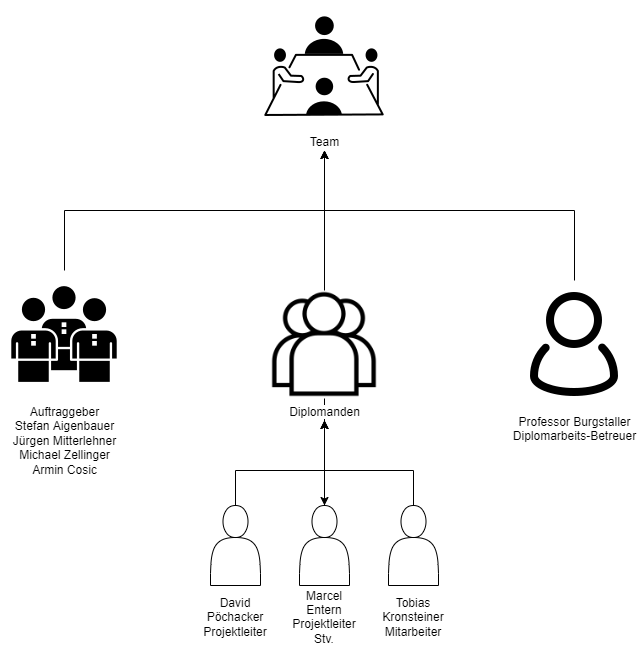
\includegraphics[height=8cm,width=8cm]{images/Team}
	\caption{Team}
	\label{fig:Team}
\end{figure}



\subsection{David Pöchacker}
Die implementierte Karte muss so konfiguriert werden, dass das Hinzufügen von Energiesystemen sowie Energietechnologien für den Benutzer möglich ist. Zusätzlich zum Erstellen eines Energiesystems oder einer Energietechnologie sollen die Funktionen, diese zu bearbeiten und zu löschen, ebenfalls gegeben sein. Um die Verwaltung der Energiesysteme unter Kontrolle zu haben und gegen unerwünschte Zugriffe zu schützen, ist ein rollenbasiertes Benutzersystem notwendig. Um diese Anforderungen zu erfüllen, müssen folgende Aufgaben umgesetzt werden:
\begin{itemize}
	\item Kartendienst Funktionen implementieren
	\item Verwaltungsfunktionen der Energiesysteme sowie Energietechnologien erstellen
	\item Benutzerverwaltungssystem einrichten
\end{itemize}



\subsection{Marcel Entner}
Hauptaufgabe ist die generelle Konzeption und Umsetzung des Front-End Designs. Er ist dafür verantwortlich, Front-End Vorlagen zu entwerfen und diese mit dem Auftraggeber abzustimmen. Das Teammitglied ist auch für die Umsetzung des Vorschlages auf der Website verantwortlich und verfasst dazu ein Designhandbuch. Eine weitere Aufgabe ist es, eine Bildergalerie, die zu jeder Energietechnologie ein dazugehöriges Bild anzeigt, zu entwerfen. Das Teammitglied  war auch dafür verantwortlich, dass eine Impressums- und eine Datenschutzseite vorhanden ist. 

\subsection{Tobias Kronsteiner}
Das Teammitglied setzt sich mit der Analyse des vorhandenen Systems sowie der Datenbank auseinander. Weiters befasst es sich mit der Analyse, Konzeption und Implementierung von Visualisierungsmöglichkeiten der anwendungsspezifischen Statistiken. Der Zugriff sowie der Datenverkehr zwischen dem Produkt und der neu konzipierten Datenbank gehört ebenfalls zum Aufgabenbereich. Zum größten Teil befasst sich das Teammitglied mit dem Visualisierungs Tool Grafana und dessen HTTP API\footnote{Anwendungsspeziefische Programmierbar Schnittstelle eines Programmes }. 
Eine besondere Herausforderung stellt hier die Implementierung eines Algorithmus zum erweitern des Datenmodells eines Dashboards \footnote{ Genauere Erklärung erfolgt im \autoref{sec: Dashboard}}. sowie das dynamische Teilen von Panels \footnote{ Genauere Erklärung erfolgt im \autoref{sec: Panels}}. auf der Benutzeroberfläche des Produktes dar. 





